\documentclass{IEEEtran}

%% Additional Packages
\usepackage{cite}
\usepackage{graphicx}
%% Macros
\newcommand{\mb}[1]{\mathbf{#1}}

\title{An FPGA Implementation of a Long Short-Term Memory Neural Network}

%% COMMENT THIS FOR SUBMISSION
\author{\IEEEauthorblockN{Jose Pedro Castro Fonseca} \\ 
\IEEEauthorblockA{Faculty of Engineering University of Porto \\
Porto, Portugal}}
\IEEEspecialpapernotice{(Working Version)}


\begin{document}

\maketitle

\begin{abstract}
This work proposes a hardware architecture for a Long Short-Term Memory (LSTM) Neural Network, aiming
to outperform software implementations, by exploiting the inherent parallelism in it.  
The main design decisions are presented, along with the proposed network architecture. A description of the main
building blocks of the network is also presented. The network is synthesized for various sizes,
and performance results are presented and analysed. The synthesized network achieves a 195 times speed-up
over a custom-built software network, proving the benefits of parallel computation for this kind of network.
\end{abstract}


\section{Introduction}\label{sec:intro}
\IEEEPARstart{N}{eural} Networks are one of the most commonly used techniques in Deep Learning. This
particular type of network, LSTM, is a recursive network, given that the neuron outputs in a certain 
time step are also fed as the input in the next time step, and that way their memory elements can make
sense of patterns within data sequences, unlike classical recursive neural networks.
These algorithms have been profusely implemented in software, and their practical applications are plentiful. 
However, the benefits of the inherent parallelism offered by a dedicated hardware
platform are not availed, and there are relatively few implementations of Machine Learning algorithms in 
these kind of platforms. 

Hardware platforms would achieve a considerable speed-up over software implementations, which could prove
useful for high data throughput systems, where the calculation overhead is critical and limits the performance of the systems.
Furthermore, a hardware implementation can even benefit \emph{offline} Deep Learning tasks by providing the results
of a given experiment faster than in a regular CPU, yielding an increase in scientific productivity.

Hitherto, there is only one implementation~\cite{Chang15}, but its performance is undermined
by the external memory access. This implementation aims to make use of internal FPGA memory resources, and therefore
achieve a higher speed performance.

In overview, this article begins by explaining what are LSTM networks -- and their mathematical details -- in Section~\ref{sec:lstmnn}, and by providing a quick overview of their state of the art in Section~\ref{sec:relwork}.
Section~\ref{sec:proparch} outlines the proposed hardware architecture and its main constituent modules, and the performance and synthesis results are reported in Section~\ref{sec:results}. A final concluding remark is given in Section~\ref{sec:concl}.

\section{LSTM Neural Networks}\label{sec:lstmnn}
Although originally formulated in~\cite{Hoch97}, its formulation has been incrementally updated in~\cite{Gers00} and~\cite{Gers2000}, and the most current version is the one in~\cite{Graves05}. One of the inital proposers of LSTM, Prof. Jürgen Schmidhüber, did a survey on the most common variations of the model last year~\cite{Greff15}, and this will the basis of this short theoretical presentation, as well as the work that will be developed in this thesis. 

A single LSTM neuron is presented in Figure~\ref{fig:lstmneuron}. As we can see from the picture, we still have the recurrent connections from the regular RNNs, but now there are multiple entry points that control the flow of information through the network. Although omitted from the picture, all the gates are biased, as is suggested in Equations~\ref{eq:equationsLSTM}. The main components, their role and relevance, are explained as follows

\begin{figure}[!t]
	\centering
	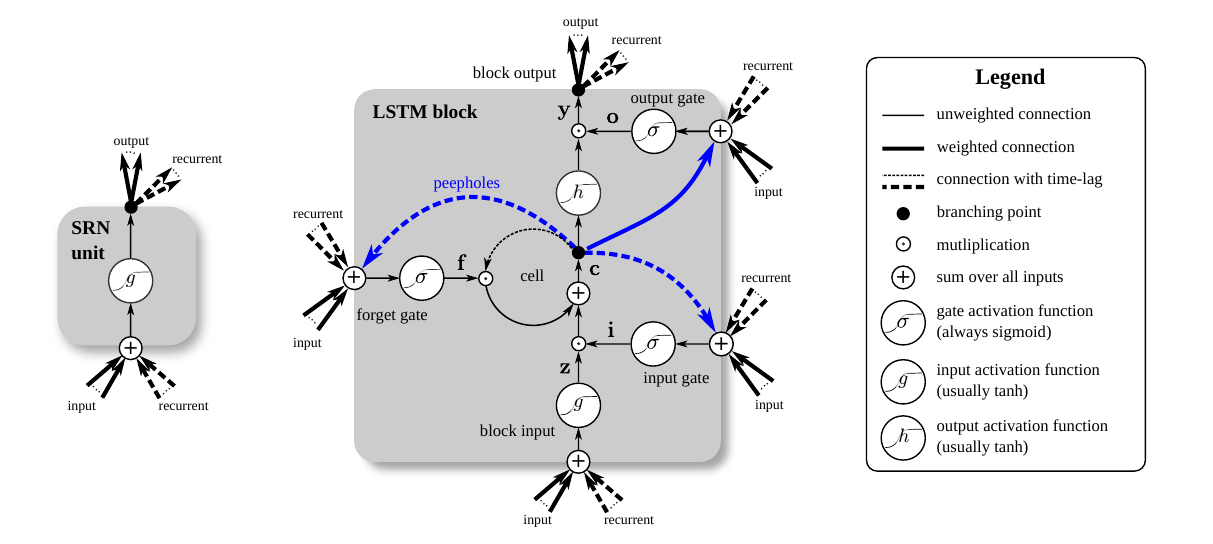
\includegraphics[width=2.5in]{figures/lstmneuron.png}
    \caption{A complete LSTM neuron, with all the features as described in~\cite{Graves05}. Source:~\cite{Greff15}}
	\label{fig:lstmneuron}
\end{figure}

\begin{itemize}
    \item \textbf{Input Gate} -- this is the input gate, where the importance of each feature of the input vector at time $t$, $\mb{x}^t$, and the output vector at the previous time step $\mb{y}^{t-1}$ is weighed in, producing an output $\mb{i}^{t}$.

    \item \textbf{Block Input Gate} -- as the name implies, this gate controls the flow of information from the input gate to the memory cell. It also receives the input vector and the previous output vector as inputs, but it does not have peephole connections and its dynamics are controlled by a different set of weights. The \textbf{activation function of this gate can be either}, but the most common choice is the \textbf{Hyperbolic Tangent}.

    \item \textbf{Forget Gate} -- its role is to control the contents of the Memory Cell, either to set them or reset them, using the \textit{Hadamard Elementwise} matrix multiplication of its output at time $t$, $\mb{c}^{(t)}$, with the contents of the memory unit at the previous time step, $\mb{c}^{(t-1)}$. The activation function of this gate is \textbf{always sigmoid}.

    \item \textbf{Output Block Gate} -- this gate has a role very similar to that of the Block Input Gate, but now it controls the information flow \textit{out} of the LSTM neuron, namely the activated Memory Cell output.

    \item \textbf{Memory Cell} -- the cornerstone of the LSTM neuron. This is the memory element of the neuron, where the previous state is kept, and updated accordingly to the dynamics of the gates that connect to it. Also, this is where the peephole connections come from. 

    \item \textbf{Output Activation} -- the output of the Memory Cell goes through this activation function that, as the gate activation function, can be any, but the \textit{hyperbolic tangent} is the most common choice.

    \item \textbf{Peepholes} -- direct connections \textit{from} the memory cell that allow for gates to `peep' at the states of the memory cell. They were added after the initial 1997 formulation, and their absence was proven to have a minimal performance impact~\cite{Greff15}.
\end{itemize}

After these small conceptual definitions, that allow us to grasp some intuition on the operation of a \textit{single} LSTM cell, I can present the overview of a \textit{layer} of LSTM neurons and their formal mathematical formulation, that will be needed both for the high-level model and the HDL description. The operation of each set of gates of the layer is given by the following set of equations

\begin{eqnarray}
    \mb{z}^{(t)} & = g(\mb{W}_z \mb{x}^{(t)} + \mb{R}_z \mb{y}^{(t-1)} + \mb{b}_z) \nonumber\\
    \mb{i}^{(t)} & = \sigma(\mb{W}_i \mb{x}^{(t)} + \mb{R}_i \mb{y}^{(t-1)} + \mb{p}_i \odot \mb{c}^{(t-1)} + \mb{b}_i) \nonumber\\
    \mb{f}^{(t)} & = \sigma(\mb{W}_f \mb{x}^{(t)} + \mb{R}_f \mb{y}^{(t-1)} + \mb{p}_f \odot \mb{c}^{(t-1)} + \mb{b}_f) \nonumber\\
    \mb{o}^{(t)} & = \sigma(\mb{W}_o \mb{x}^{(t)} + \mb{R}_o \mb{y}^{(t-1)} + \mb{p}_o \odot \mb{c}^{(t)} + \mb{b}_o) \nonumber\\
    \mb{c}^{(t)} & = \mb{i}^{(t)} \odot \mb{z}^{(t)} + \mb{f}^{(t)} \odot \mb{c}^{(t-1)} \nonumber \\
    \mb{y}^{(t)} & = \mb{o}^{(t)} \odot h(\mb{z}^{(t)}) \label{eq:equationsLSTM}
\end{eqnarray}
where $\odot$ is the Hadamard multiplication. The $i$-th element of the previous vectors in bold corresponds to the value of the gate of the $i$-th neuron of the layer, which is a very convenient and compact representation of the whole layer. Furthermore, if the layer has $N$ LSTM neurons and $M$ inputs (i.e. the size of the layer that precedes this), we see that the input weight matrices $\mb{W}_*$ and the  recurrent weight matrices $\mb{R}_*$ all have size $N \times M$, and that the bias weight matrices $\mb{b}_*$, the peephole weight matrices $\mb{p}_*$ and the matrices $\mb{z}^{(t)}$ through $\mb{c}^{(t)}$ have size $N \times 1$.

\section{Related Work}\label{sec:relwork}

\section{Proposed Architecture}\label{sec:proparch}

\subsection{Activation Function Calculation}

\subsection{Matrix-vector Dot Product Calculation}

\subsection{Weight storage}

\subsection{Network Architecture}

\section{Results}\label{sec:results}

\subsection{Validation}

\subsection{Synthesis}

\subsection{Performance}

\section{Conclusion}\label{sec:concl}

\bibliographystyle{IEEEtran}  
\bibliography{bibliography} 

\end{document}
